\section{Introduction}
\label{section:intro}

\begin{figure*}[t]
    \centering
    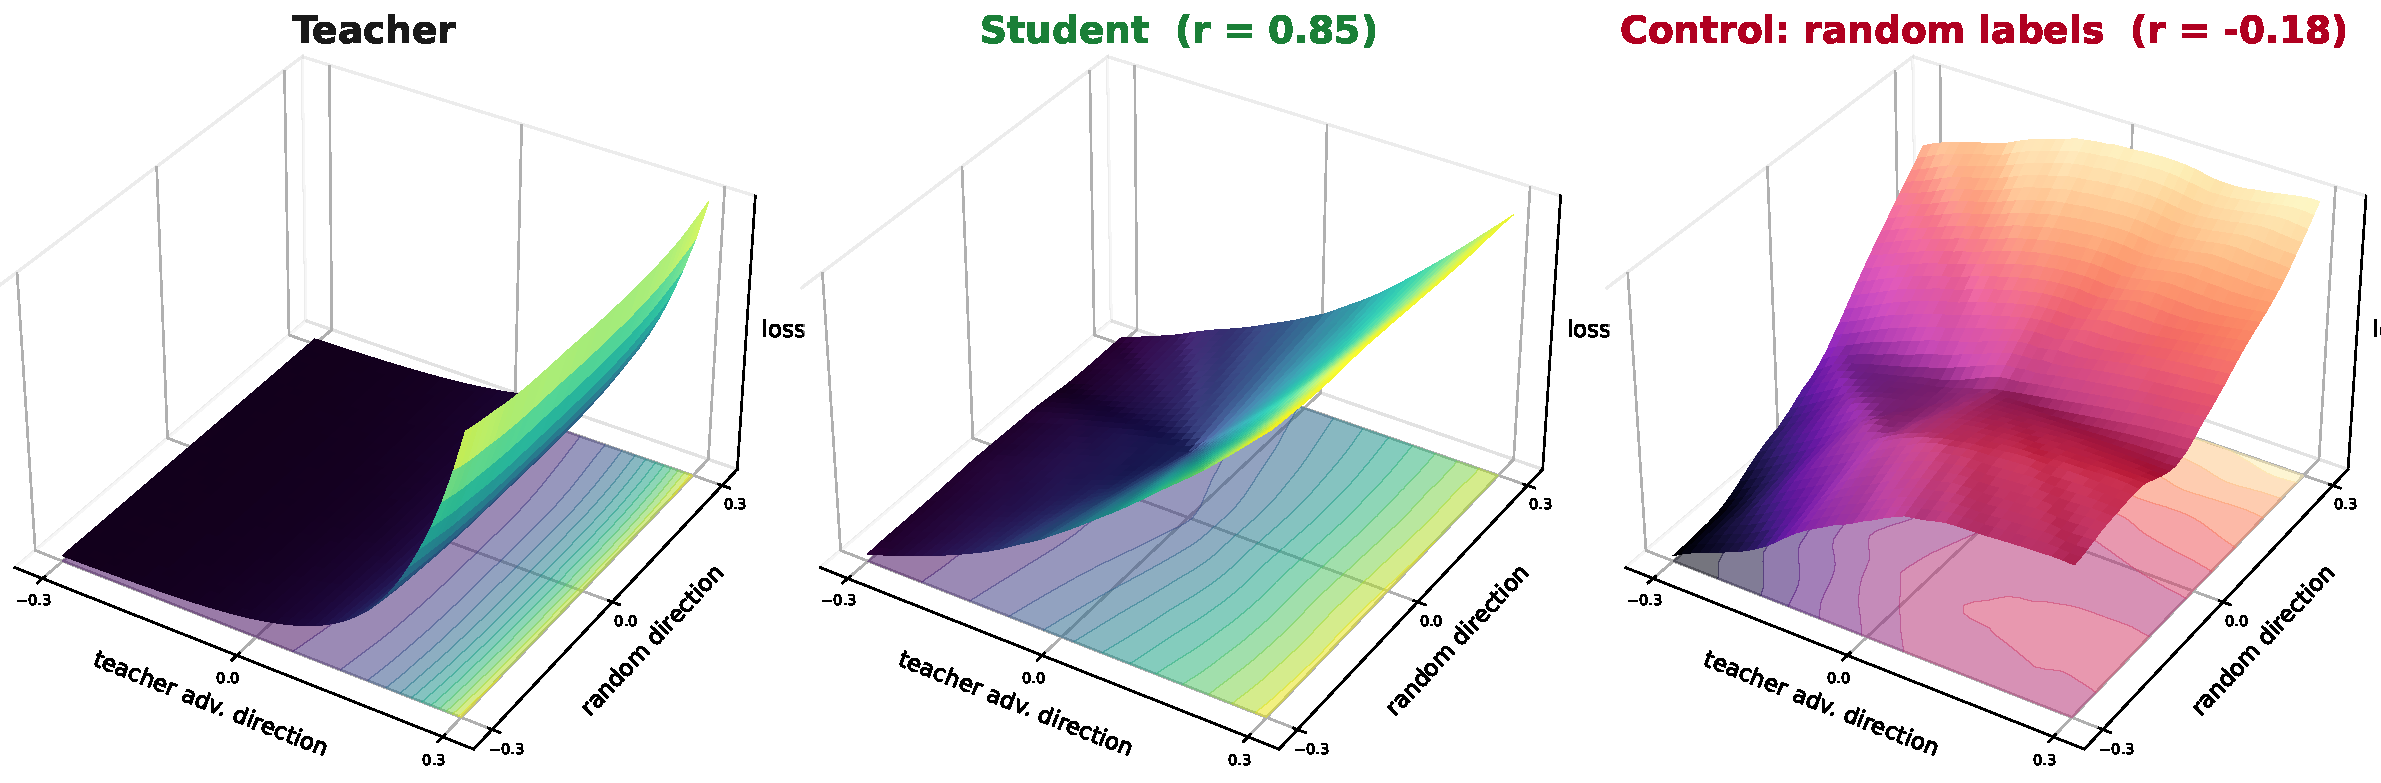
\includegraphics[width=0.95\textwidth]{imgs/teaser_loss_landscape_3d.pdf}
    \caption{Adversarial loss landscapes for a teacher, a student distilled solely on Gaussian noise (no ground-truth labels), and a destroy-the-signal control, evaluated on an MNIST test digit. Each surface plots cross-entropy loss over a $\pm 0.3\,L_{\infty}$ neighborhood spanned by the teacher's adversarial gradient direction and an orthogonal random direction; loss is normalised per panel so shapes are directly comparable. When subliminal learning occurs, the student reproduces the teacher's sharp adversarial ridge $(r = 0.85)$, whereas a control trained identically but on random soft labels does not $(r = -0.18)$ -- showing the adversarial geometry is inherited through the genuine distillation signal rather than the shared architecture or training procedure.}
    \label{fig:teaser_loss}
\end{figure*}

\textbf{Knowledge Distillation and Transfer Risks
} 
Knowledge distillation → transfers model capabilities → must isolate only the intended safe capabilities or only specific tasks  → because LLMs may also contain harmful side effects → such as adversarial vulnerabilities, fake alignment, and reward hacking → therefore, we need to verify exactly what knowledge is transferred.

\textbf{Adversarial Space and Transferability.} 
Latent space -> Features decomposition -> Also Adversarial space → DNNs contain adversarial slopes and features decomposition  → these can be expressed through output signals  → therefore, during distillation, the student may convergence into  the teacher’s latent space, including the adversarial space rather than only the intended task knowledge.



\textbf{Current Work and Knowledge Gaps.} Problematic knowledge transmission → prior distillation studies show that  traits can pass in distillation → \textbf{GAP:} 


Knowledge distillation is usually understood as a procedure for transferring \emph{visible} task behavior from a teacher model to a student model. Recent work on \emph{subliminal learning}, however, shows that teacher-generated data can transmit hidden traits even when the generated data is semantically unrelated to those traits. This motivates a broader question: does distillation transfer only observable input--output behavior, or can it also transmit deeper latent structure? We call this broader phenomenon \emph{latent teleportation}: the transmission of teacher-specific latent geometry to a student through hidden signals embedded in generated or distilled data.

In this work we study whether distillation transmits feature geometry, steering vectors, adversarial structure, and training-induced internal modifications. Our focus is not a single copied vulnerability or a single copied behavior, but whether the student's internal representation becomes aligned with the teacher's latent and adversarial geometry after learning only from teacher-generated data. The structural backbone of our analysis is the observation that the student approximates the teacher within the parameter subspace encoded by hidden signals in the distilled data; each individual finding then follows as an instantiation of a single observable approximation lemma, obtained by reading this parameter-level statement through a different observable. Our main contributions are as follows:

\begin{itemize}
    \item \textbf{Formalizing latent teleportation.} We introduce and formalize latent teleportation, deriving from first principles that distillation aligns the student with the teacher in the subspace carried by hidden signals in generated data, and we show that feature, adversarial, and behavioral transfer all reduce to one observable approximation lemma.
    \item \textbf{Transfer of latent feature and adversarial geometry.} We show that a student trained only on teacher-generated data inherits the teacher's internal geometry: teacher-derived steering vectors steer the student class-by-class, representations align on arbitrary inputs, and adversarial slopes, optimization trajectories, attack-induced latent shifts, and teacher-crafted targeted attacks all transfer to the student.
    \item \textbf{Transfer of training-induced modifications and controls.} We show that deliberate teacher-side modifications---injected knowledge, secondary behavioral side effects, and aggregate safety/refusal tendencies---are transmitted to the student through generated data alone, and we verify with base, independent, different-initialization, and corrupted-data controls that these effects reflect hidden-signal transmission rather than ordinary imitation or evaluation artifacts.
    \end{itemize}
